\lettrine[lhang=0.17]{I}{t} seems like in category theory everything is related to everything and
everything can be viewed from many angles. Take for instance the
universal construction of the \namelink{chap:0105}{product}.
Now that we know more about \namelink{chap:0107}{functors} and
\namelink{chap:0110}{natural transformations}, can we simplify and, possibly, generalize it? Let us
try.

\begin{figure}[H]
    \centering
    \fbox{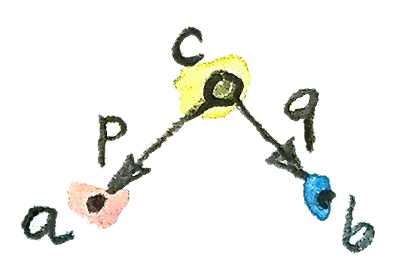
\includegraphics[width=1.56250in]{images/productpattern.jpg}}
\end{figure}

The construction of a product starts with the selection of two objects
\texttt{a} and \texttt{b}, whose product we want to construct. But what
does it mean to \emph{select objects}? Can we rephrase this action in
more categorical terms? Two objects form a pattern --- a very simple
pattern. We can abstract this pattern into a category --- a very simple
category, but a category nevertheless. It's a category that we'll call
\mathtext{2}. It contains just two objects, 1 and 2, and no morphisms
other than the two obligatory identities. Now we can rephrase the
selection of two objects in \mathtext{C} as the act of defining a functor \mathtext{D}
from the category \mathtext{2} to \mathtext{C}. A functor maps objects to
objects, so its image is just two objects (or it could be one, if the
functor collapses objects, which is fine too). It also maps morphisms
--- in this case it simply maps identity morphisms to identity
morphisms.

\begin{figure}[H]
    \centering
    \fbox{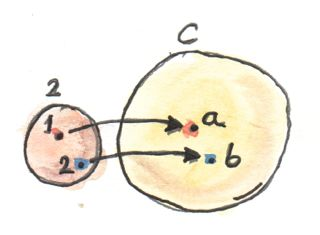
\includegraphics[width=1.56250in]{images/two.jpg}}
\end{figure}

What's great about this approach is that it builds on categorical
notions, eschewing the imprecise descriptions like "selecting
objects", taken straight from the hunter-gatherer lexicon of our
ancestors. And, incidentally, it is also easily generalized, because
nothing can stop us from using categories more complex than \mathtext{2}
to define our patterns.

But let's continue. The next step in the definition of a product is the
selection of the candidate object \mathtext{c}. Here again, we could
rephrase the selection in terms of a functor from a singleton category.
And indeed, if we were using Kan extensions, that would be the right
thing to do. But since we are not ready for Kan extensions yet, there is
another trick we can use: a constant functor \mathtext{\Delta} from the same category
\mathtext{2} to \mathtext{C}. The selection of \mathtext{c} in \mathtext{C} can be
done with \mathtext{\Delta_c}. Remember, \mathtext{\Delta_c} maps all
objects into \mathtext{c} and all morphisms into \mathtext{id_c}.

\begin{figure}[H]
    \centering
    \fbox{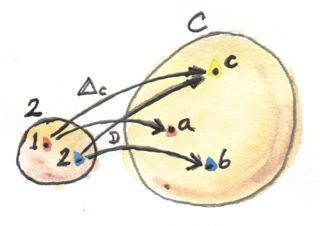
\includegraphics[width=1.56250in]{images/twodelta.jpg}}
\end{figure}

Now we have two functors, \mathtext{\Delta_c} and \mathtext{D} going between
\mathtext{2} and \mathtext{C} so it's only natural to ask about natural
transformations between them. Since there are only two objects in
\mathtext{2}, a natural transformation will have two components. Object 1
in \mathtext{2} is mapped to \mathtext{c} by \mathtext{\Delta_c} and to
\mathtext{a} by \mathtext{D}. So the component of a natural transformation between
\mathtext{\Delta_c} and \mathtext{D} at \mathtext{1} is a morphism from \mathtext{c} to
\mathtext{a}. We can call it \mathtext{p}. Similarly, the second component
is a morphism \mathtext{q} from \mathtext{c} to \mathtext{b} --- the image of
the object 2 in \mathtext{2} under \mathtext{D}. But these are exactly like the two
projections we used in our original definition of the product. So
instead of talking about selecting objects and projections, we can just
talk about picking functors and natural transformations. It so happens
that in this simple case the naturality condition for our transformation
is trivially satisfied, because there are no morphisms (other than the
identities) in \mathtext{2}.

\begin{figure}[H]
    \centering
    \fbox{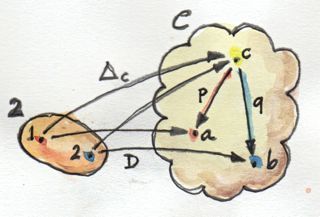
\includegraphics[width=1.56250in]{images/productcone.jpg}}
\end{figure}

A generalization of this construction to categories other than
\mathtext{2} --- ones that, for instance, contain non-trivial morphisms
--- will impose naturality conditions on the transformation between
\mathtext{\Delta_c} and \mathtext{D}. We call such transformation a \emph{cone},
because the image of \mathtext{\Delta} is the apex of a cone/pyramid whose sides are
formed by the components of the natural transformation. The image of \mathtext{D}
forms the base of the cone.

In general, to build a cone, we start with a category \mathtext{I} that
defines the pattern. It's a small, often finite category. We pick a
functor \mathtext{D} from \mathtext{I} to \mathtext{C} and call it (or its image) a
\emph{diagram}. We pick some \mathtext{c} in \mathtext{C} as the apex of our
cone. We use it to define the constant functor \mathtext{\Delta_c} from
\mathtext{I} to \mathtext{C}. A natural transformation from \mathtext{\Delta_c}
to \mathtext{D} is then our cone. For a finite \mathtext{I} it's just a bunch of
morphisms connecting \mathtext{c} to the diagram: the image of \mathtext{I}
under \mathtext{D}.

\begin{figure}[H]
    \centering
    \fbox{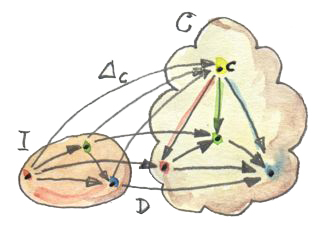
\includegraphics[width=1.56250in]{images/cone.jpg}}
\end{figure}

Naturality requires that all triangles (the walls of the pyramid) in
this diagram commute. Indeed, take any morphism \mathtext{f} in \mathtext{I}.
The functor \mathtext{D} maps it to a morphism \mathtext{D f} in \mathtext{C}, a
morphism that forms the base of some triangle. The constant functor
\mathtext{\Delta_c} maps \mathtext{f} to the identity morphism on
\mathtext{c}. \mathtext{\Delta} squishes the two ends of the morphism into one object, and
the naturality square becomes a commuting triangle. The two arms of this
triangle are the components of the natural transformation.

\begin{figure}[H]
    \centering
    \fbox{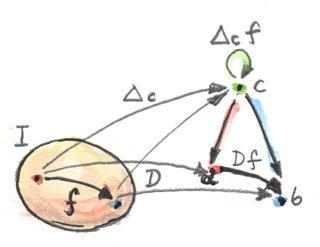
\includegraphics[width=1.56250in]{images/conenaturality.jpg}}
\end{figure}

So that's one cone. What we are interested in is the \emph{universal
cone} --- just like we picked a universal object for our definition of a
product.

There are many ways to go about it. For instance, we may define a
\emph{category of cones} based on a given functor \mathtext{D}. Objects in that
category are cones. Not every object \mathtext{c} in \mathtext{C} can be an
apex of a cone, though, because there may be no natural transformation
between \mathtext{\Delta_c} and \mathtext{D}.

To make it a category, we also have to define morphisms between cones.
These would be fully determined by morphisms between their apexes. But
not just any morphism will do. Remember that, in our construction of the
product, we imposed the condition that the morphisms between candidate
objects (the apexes) must be common factors for the projections. For
instance:

\begin{equation*}
\begin{split}
p' = p \cdot m \\
q' = q \cdot m
\end{split}
\end{equation*}

\begin{figure}[H]
    \centering
    \fbox{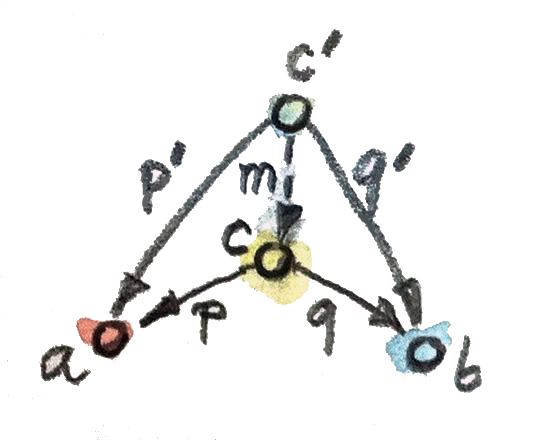
\includegraphics[width=1.56250in]{images/productranking.jpg}}
\end{figure}

This condition translates, in the general case, to the condition that
the triangles whose one side is the factorizing morphism all commute.

\begin{figure}[H]
    \centering
    \fbox{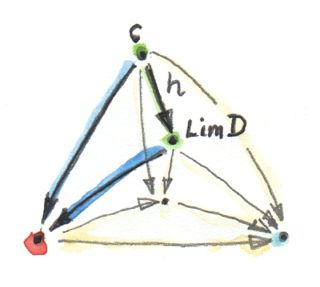
\includegraphics[width=2.48958in]{images/conecommutativity.jpg}}
    \captionsetup{labelformat=empty,font=scriptsize}
    \caption{The commuting triangle connecting two cones, with the factorizing
morphism \code{h} (here, the lower cone is the universal one, with
\code{Lim D} as its apex)}
\end{figure}

We'll take those factorizing morphisms as the morphisms in our category
of cones. It's easy to check that those morphisms indeed compose, and
that the identity morphism is a factorizing morphism as well. Cones
therefore form a category.

Now we can define the universal cone as the \emph{terminal object} in
the category of cones. The definition of the terminal object states that
there is a unique morphism from any other object to that object. In our
case it means that there is a unique factorizing morphism from the apex
of any other cone to the apex of the universal cone. We call this
universal cone the \emph{limit} of the diagram \mathtext{D}, \code{Lim D} (in
the literature, you'll often see a left arrow pointing towards \mathtext{I}
under the \mathtext{Lim} sign). Often, as a shorthand, we call the apex of
this cone the limit (or the limit object).

The intuition is that the limit embodies the properties of the whole
diagram in a single object. For instance, the limit of our two-object
diagram is the product of two objects. The product (together with the
two projections) contains the information about both objects. And being
universal means that it has no extraneous junk.

\subsection{Limit as a Natural Isomorphism}\label{limit-as-a-natural-isomorphism}

There is still something unsatisfying about this definition of a limit.
I mean, it's workable, but we still have this commutativity condition
for the triangles that are linking any two cones. It would be so much
more elegant if we could replace it with some naturality condition. But
how?

We are no longer dealing with one cone but with a whole collection (in
fact, a category) of cones. If the limit exists (and --- let's make it
clear --- there's no guarantee of that), one of those cones is the
universal cone. For every other cone we have a unique factorizing
morphism that maps its apex, let's call it \mathtext{c}, to the apex of
the universal cone, which we named \code{Lim D}. (In fact, I can skip
the word "other", because the identity morphism maps the universal
cone to itself and it trivially factorizes through itself.) Let me
repeat the important part: given any cone, there is a unique morphism of
a special kind. We have a mapping of cones to special morphisms, and
it's a one-to-one mapping.

This special morphism is a member of the hom-set \code{C(c, LimD)}.
The other members of this hom-set are less fortunate, in the sense that
they don't factorize the mapping of cones. What we want is to be able to
pick, for each \code{c}, one morphism from the set
\code{C(c, LimD)} --- a morphism that satisfies the particular
commutativity condition. Does that sound like defining a natural
transformation? It most certainly does!

But what are the functors that are related by this transformation?

One functor is the mapping of \code{c} to the set
\code{C(c, Lim D)}. It's a functor from \mathtext{C} to \textbf{Set} ---
it maps objects to sets. In fact it's a contravariant functor. Here's
how we define its action on morphisms: Let's take a morphism \code{f}
from \code{c'} to \code{c}:

\mint{haskell}|f :: c' -> c|

Our functor maps \code{c'} to the set
\code{C(c', Lim D)}. To define the action of this functor on
\code{f} (in other words, to lift \code{f}), we have to define the
corresponding mapping between \code{C(c, Lim D)} and
\code{C(c', Lim D)}. So let's pick one element \code{u} of
\code{C(c, Lim D)} and see if we can map it to some element of
\code{C(c', Lim D)}. An element of a hom-set is a morphism, so
we have:

\mint{haskell}|u :: c -> Lim D|

We can precompose \code{u} with \code{f} to get:

\mint{haskell}|u . f :: c' -> Lim D|

And that's an element of \code{C(c', Lim D)}--- so indeed, we
have found a mapping of morphisms:

\begin{minted}{haskell}
contramap :: (c' -> c) -> (c -> Lim D) -> (c' -> Lim D) 
contramap f u = u . f
\end{minted}

Notice the inversion in the order of \code{c} and \code{c'}
characteristic of a \emph{contravariant} functor.

\begin{figure}[H]
    \centering
    \fbox{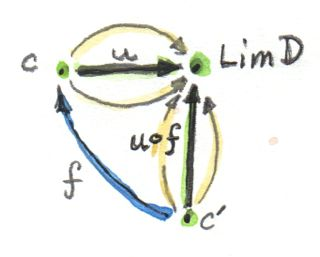
\includegraphics[width=2.59375in]{images/homsetmapping.jpg}}
\end{figure}

To define a natural transformation, we need another functor that's also
a mapping from \mathtext{C} to \mathtext{Set}. But this time we'll consider a
set of cones. Cones are just natural transformations, so we are looking
at the set of natural transformations \code{Nat(\ensuremath{\Delta_c} D)}. The mapping
from \code{c} to this particular set of natural transformations is a
(contravariant) functor. How can we show that? Again, let's define its
action on a morphism:

\mint{haskell}|f :: c' -> c|

The lifting of \code{f} should be a mapping of natural transformations
between two functors that go from \mathtext{I} to \mathtext{C}:

\begin{minted}[escapeinside=||,mathescape=true]{haskell}
Nat(|\ensuremath{\Delta_c}|, D) -> Nat(|\ensuremath{\Delta_{c'}}|, D)
\end{minted}

How do we map natural transformations? Every natural transformation is a
selection of morphisms --- its components --- one morphism per element
of \mathtext{I}. A component of some \mathtext{\alpha} (a member of \code{ Nat(\ensuremath{\Delta_c}, D)}) at
\code{a} (an object in \mathtext{I}) is a morphism:

\begin{minted}[escapeinside=||,mathescape=true]{haskell}
|\ensuremath{\alpha_a}|:: |\ensuremath{\Delta_c a}| -> D a
\end{minted}

or, using the definition of the constant functor \mathtext{\Delta},

\begin{minted}[escapeinside=||,mathescape=true]{haskell}
|\ensuremath{\alpha_a}| :: c -> D a
\end{minted}

Given \code{f} and \mathtext{\alpha}, we have to construct a \mathtext{\beta}, a member of
\code{Nat(\ensuremath{\Delta_{c'}},\ D)}. Its component at \code{a} should be a
morphism:

\begin{minted}[escapeinside=||,mathescape=true]{haskell}
|\ensuremath{\beta_a}| :: c' -> D a
\end{minted}

We can easily get the latter from the former by precomposing it with
\code{f}:

\begin{minted}[escapeinside=||,mathescape=true]{haskell}
|\ensuremath{\beta_a}| = |\ensuremath{\alpha_a}| . f
\end{minted}


It's relatively easy to show that those components indeed add up to a
natural transformation.

\begin{figure}[H]
    \centering
    \fbox{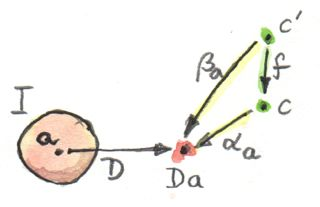
\includegraphics[width=1.56250in]{images/natmapping.jpg}}
\end{figure}

Given our morphism \code{f}, we have thus built a mapping between two
natural transformations, component-wise. This mapping defines
\code{contramap} for the functor:

\begin{minted}[escapeinside=||,mathescape=true]{haskell}
c -> Nat(|\ensuremath{\Delta_c}|, D)
\end{minted}

What I have just done is to show you that we have two (contravariant)
functors from \mathtext{C} to \textbf{Set}. I haven't made any assumptions
--- these functors always exist.

Incidentally, the first of these functors plays an important role in
category theory, and we'll see it again when we talk about Yoneda's
lemma. There is a name for contravariant functors from any category
\mathtext{C} to \textbf{Set}: they are called "presheaves". This one is
called a \emph{representable presheaf}. The second functor is also a
presheaf.

Now that we have two functors, we can talk about natural transformations
between them. So without further ado, here's the conclusion: A functor
\code{D} from \mathtext{I} to \mathtext{C} has a limit \code{Lim D} if and
only if there is a natural isomorphism between the two functors I have
just defined:

\begin{minted}[escapeinside=||,mathescape=true]{haskell}
C(c, Lim D) |\ensuremath{\backsimeq}| Nat(|\ensuremath{\Delta_c}|, D)
\end{minted}

Let me remind you what a natural isomorphism is. It's a natural
transformation whose every component is an isomorphism, that is to say
an invertible morphism.

I'm not going to go through the proof of this statement. The procedure
is pretty straightforward if not tedious. When dealing with natural
transformations, you usually focus on components, which are morphisms.
In this case, since the target of both functors is \textbf{Set}, the
components of the natural isomorphism will be functions. These are
higher order functions, because they go from the hom-set to the set of
natural transformations. Again, you can analyze a function by
considering what it does to its argument: here the argument will be a
morphism --- a member of \code{C(c, Lim D)} --- and the result will
be a natural transformation --- a member of \code{Nat(\ensuremath{\Delta_c}, D)}, or
what we have called a cone. This natural transformation, in turn, has
its own components, which are morphisms. So it's morphisms all the way
down, and if you can keep track of them, you can prove the statement.

The most important result is that the naturality condition for this
isomorphism is exactly the commutativity condition for the mapping of
cones.

As a preview of coming attractions, let me mention that the set
\code{Nat(\ensuremath{\Delta_c}, D)} can be thought of as a hom-set in the functor
category; so our natural isomorphism relates two hom-sets, which points
at an even more general relationship called an adjunction.

\subsection{Examples of Limits}\label{examples-of-limits}

We've seen that the categorical product is a limit of a diagram
generated by a simple category we called \mathtext{2}.

There is an even simpler example of a limit: the terminal object. The
first impulse would be to think of a singleton category as leading to a
terminal object, but the truth is even starker than that: the terminal
object is a limit generated by an empty category. A functor from an
empty category selects no object, so a cone shrinks to just the apex.
The universal cone is the lone apex that has a unique morphism coming to
it from any other apex. You will recognize this as the definition of the
terminal object.

The next interesting limit is called the \emph{equalizer}. It's a limit
generated by a two-element category with two parallel morphisms going
between them (and, as always, the identity morphisms). This category
selects a diagram in \mathtext{C} consisting of two objects, \code{a} and
\code{b}, and two morphisms:

\begin{minted}[escapeinside=||,mathescape=true]{haskell}
f :: a -> b 
g :: a -> b
\end{minted}

To build a cone over this diagram, we have to add the apex, \texttt{c}
and two projections:

\begin{minted}[escapeinside=||,mathescape=true]{haskell}
p :: c -> a 
q :: c -> b
\end{minted}

\begin{figure}[H]
    \centering
    \fbox{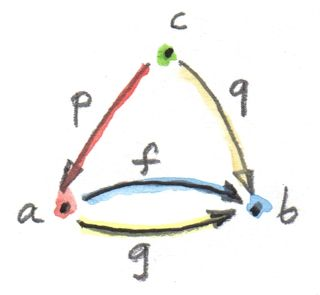
\includegraphics[width=2.27083in]{images/equalizercone.jpg}}
\end{figure}

We have two triangles that must commute:

\begin{minted}[escapeinside=||,mathescape=true]{haskell}
q = f . p 
q = g . p
\end{minted}

This tells us that \code{q} is uniquely determined by one of these
equations, say, \code{q = f . p}, and we can omit it from the
picture. So we are left with just one condition:

\begin{minted}[escapeinside=||,mathescape=true]{haskell}
f . p = g . p
\end{minted}

The way to think about it is that, if we restrict our attention to
\textbf{Set}, the image of the function \texttt{p} selects a subset of
\code{a}. When restricted to this subset, the functions \code{f} and
\code{g} are equal.

For instance, take \code{a} to be the two-dimensional plane
parameterized by coordinates \code{x} and \code{y}. Take \code{b}
to be the real line, and take:

\begin{minted}[escapeinside=||,mathescape=true]{haskell}
f (x, y) = 2 * y + x 
g (x, y) = y - x
\end{minted}

The equalizer for these two functions is the set of real numbers (the
apex, \code{c}) and the function:

\begin{minted}[escapeinside=||,mathescape=true]{haskell}
p t = (t, (-2) * t)
\end{minted}

Notice that \code{(p t)} defines a straight line in the
two-dimensional plane. Along this line, the two functions are equal.

Of course, there are other sets \code{c'} and functions
\texttt{p'} that may lead to the equality:

\begin{minted}[escapeinside=||,mathescape=true]{haskell}
f . p' = g . p'
\end{minted}

but they all uniquely factor out through \texttt{p}. For instance, we
can take the singleton set \texttt{()} as \texttt{c\&apos;} and the
function:

\begin{minted}[escapeinside=||,mathescape=true]{haskell}
p'() = (0, 0)
\end{minted}

It's a good cone, because \code{f (0, 0) = g (0, 0)}. But it's
not universal, because of the unique factorization through \code{h}:

\begin{minted}[escapeinside=||,mathescape=true]{haskell}
p' = p . h
\end{minted}

with

\begin{minted}[escapeinside=||,mathescape=true]{haskell}
h () = 0
\end{minted}

\begin{figure}[H]
    \centering
    \fbox{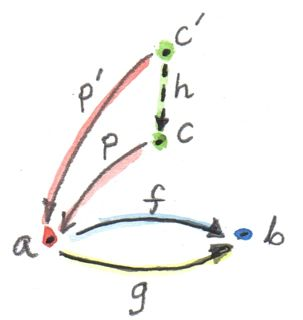
\includegraphics[width=2.19792in]{images/equilizerlimit.jpg}}
\end{figure}

An equalizer can thus be used to solve equations of the type
\code{f x = g x}. But it's much more general, because it's defined
in terms of objects and morphisms rather than algebraically.

An even more general idea of solving an equation is embodied in another
limit --- the pullback. Here, we still have two morphisms that we want
to equate, but this time their domains are different. We start with a
three-object category of the shape:
\code{1-\textgreater{}2\textless{}-3}. The diagram corresponding to
this category consists of three objects, \code{a}, \code{b}, and
\code{c}, and two morphisms:

\begin{minted}[escapeinside=||,mathescape=true]{haskell}
f :: a -> b 
g :: c -> b
\end{minted}

This diagram is often called a \emph{cospan}.

A cone built on top of this diagram consists of the apex, \texttt{d},
and three morphisms:

\begin{minted}[escapeinside=||,mathescape=true]{haskell}
p :: d -> a 
q :: d -> c 
r :: d -> b
\end{minted}

\begin{figure}[H]
    \centering
    \fbox{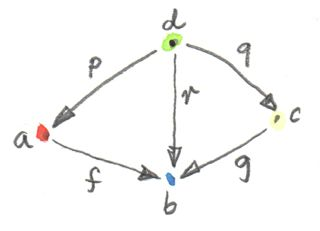
\includegraphics[width=2.47917in]{images/pullbackcone.jpg}}
\end{figure}

Commutativity conditions tell us that \code{r} is completely
determined by the other morphisms, and can be omitted from the picture.
So we are only left with the following condition:

\begin{minted}[escapeinside=||,mathescape=true]{haskell}
g . q = f . p
\end{minted}

A pullback is a universal cone of this shape.

\begin{figure}[H]
    \centering
    \fbox{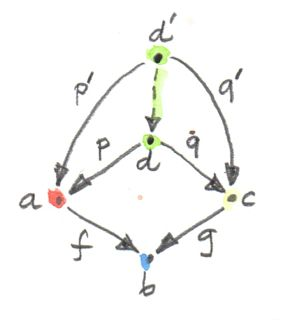
\includegraphics[width=2.12500in]{images/pullbacklimit.jpg}}
\end{figure}

Again, if you narrow your focus down to sets, you can think of the
object \code{d} as consisting of pairs of elements from \code{a} and
\code{c} for which \code{f} acting on the first component is equal
to \code{g} acting on the second component. If this is still too
general, consider the special case in which \code{g} is a constant
function, say \code{g \_ = 1.23} (assuming that \code{b} is a set
of real numbers). Then you are really solving the equation:

\begin{minted}[escapeinside=||,mathescape=true]{haskell}
f x = 1.23
\end{minted}

In this case, the choice of \code{c} is irrelevant (as long as it's
not an empty set), so we can take it to be a singleton set. The set
\code{a} could, for instance, be the set of three-dimensional vectors,
and \code{f} the vector length. Then the pullback is the set of pairs
\code{(v, ())}, where \code{v} is a vector of length 1.23 (a
solution to the equation \code{sqrt (\ensuremath{x^2+y^2+z^2}) = 1.23}), and
\code{()} is the dummy element of the singleton set.

But pullbacks have more general applications, also in programming. For
instance, consider C++ classes as a category in which morphism are
arrows that connect subclasses to superclasses. We'll consider
inheritance a transitive property, so if C inherits from B and B
inherits from A then we'll say that C inherits from A (after all, you
can pass a pointer to C where a pointer to A is expected). Also, we'll
assume that C inherits from C, so we have the identity arrow for every
class. This way subclassing is aligned with subtyping. C++ also supports
multiple inheritance, so you can construct a diamond inheritance diagram
with two classes B and C inheriting from A, and a fourth class D
multiply inheriting from B and C. Normally, D would get two copies of A,
which is rarely desirable; but you can use virtual inheritance to have
just one copy of A in D.

What would it mean to have D be a pullback in this diagram? It would
mean that any class E that multiply inherits from B and C is also a
subclass of D. This is not directly expressible in C++, where subtyping
is nominal (the C++ compiler wouldn't infer this kind of class
relationship --- it would require "duck typing"). But we could go
outside of the subtyping relationship and instead ask whether a cast
from E to D would be safe or not. This cast would be safe if D were the
bare-bone combination of B and C, with no additional data and no
overriding of methods. And, of course, there would be no pullback if
there is a name conflict between some methods of B and C.

\begin{figure}[H]
    \centering
    \fbox{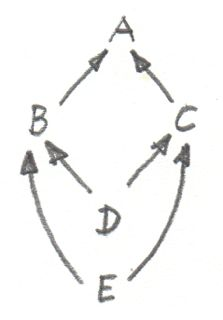
\includegraphics[width=1.61458in]{images/classes.jpg}}
\end{figure}

There's also a more advanced use of a pullback in type inference. There
is often a need to \emph{unify} types of two expressions. For instance,
suppose that the compiler wants to infer the type of a function:

\begin{minted}[escapeinside=||,mathescape=true]{haskell}
twice f x = f (f x)
\end{minted}

It will assign preliminary types to all variables and sub-expressions.
In particular, it will assign:

\begin{minted}[escapeinside=||,mathescape=true]{haskell}
f       :: t0 
x       :: t1 
f x     :: t2 
f (f x) :: t3
\end{minted}

from which it will deduce that:

\begin{minted}[escapeinside=||,mathescape=true]{haskell}
twice :: t0 -> t1 -> t3
\end{minted}

It will also come up with a set of constraints resulting from the rules
of function application:

\begin{minted}[escapeinside=||,mathescape=true]{haskell}
t0 = t1 -> t2 -- because f is applied to x 
t0 = t2 -> t3 -- because f is applied to (f x)
\end{minted}

These constraints have to be unified by finding a set of types (or type
variables) that, when substituted for the unknown types in both
expressions, produce the same type. One such substitution is:

\begin{minted}[escapeinside=||,mathescape=true]{haskell}
t1 = t2 = t3 = Int 
twice :: (Int -> Int) -> Int -> Int
\end{minted}

but, obviously, it's not the most general one. The most general
substitution is obtained using a pullback. I won't go into the details,
because they are beyond the scope of this book, but you can convince
yourself that the result should be:

\begin{minted}[escapeinside=||,mathescape=true]{haskell}
twice :: (t -> t) -> t -> t
\end{minted}

with \code{t} a free type variable.

\subsection{Colimits}\label{colimits}

Just like all constructions in category theory, limits have their dual
image in opposite categories. When you invert the direction of all
arrows in a cone, you get a co-cone, and the universal one of those is
called a colimit. Notice that the inversion also affects the factorizing
morphism, which now flows from the universal co-cone to any other
co-cone.

\begin{figure}[H]
    \centering
    \fbox{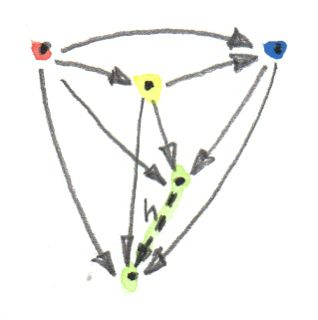
\includegraphics{images/colimit.jpg}}
\end{figure}

Cocone with a factorizing morphism \code{h} connecting two apexes.

A typical example of a colimit is a coproduct, which corresponds to the
diagram generated by \textbf{2}, the category we've used in the
definition of the product.

\begin{figure}[H]
    \centering
    \fbox{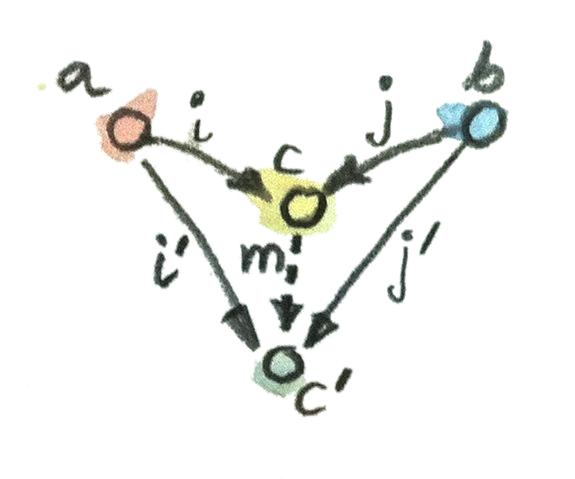
\includegraphics[width=1.56250in]{images/coproductranking.jpg}}
\end{figure}

Both the product and the coproduct embody the essence of a pair of
objects, each in a different way.

Just like the terminal object was a limit, so the initial object is a
colimit corresponding to the diagram based on an empty category.

The dual of the pullback is called the \emph{pushout}. It's based on a
diagram called a span, generated by the category
\texttt{1\textless{}-2-\textgreater{}3}.

\subsection{Continuity}\label{continuity}

I said previously that functors come close to the idea of continuous
mappings of categories, in the sense that they never break existing
connections (morphisms). The actual definition of a \emph{continuous
functor} \code{F} from a category \mathtext{C} to \mathtext{C'} includes the
requirement that the functor preserve limits. Every diagram \texttt{D}
in \emph{C} can be mapped to a diagram \mathtext{F \circ D} in \mathtext{C'} by
simply composing two functors. The continuity condition for \mathtext{F}
states that, if the diagram \mathtext{D} has a limit \code{Lim D}, then
the diagram \mathtext{F \circ D} also has a limit, and it is equal to
\code{F (Lim D)}.

\begin{figure}[H]
    \centering
    \fbox{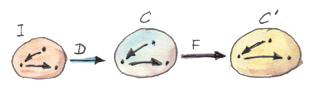
\includegraphics[width=3.12500in]{images/continuity.jpg}}
\end{figure}

Notice that, because functors map morphisms to morphisms, and
compositions to compositions, an image of a cone is always a cone. A
commuting triangle is always mapped to a commuting triangle (functors
preserve composition). The same is true for the factorizing morphisms:
the image of a factorizing morphism is also a factorizing morphism. So
every functor is \emph{almost} continuous. What may go wrong is the
uniqueness condition. The factorizing morphism in \mathtext{C'} might not be
unique. There may also be other ``better cones'' in \mathtext{C'} that were
not available in \mathtext{C}.

A hom-functor is an example of a continuous functor. Recall that the
hom-functor, \code{C(a, b)}, is contravariant in the first variable
and covariant in the second. In other words, it's a functor:

\begin{minted}[escapeinside=||,mathescape=true]{haskell}
|\ensuremath{C^{op}} \times C| -> Set
\end{minted}

When its second argument is fixed, the hom-set functor (which becomes
the representable presheaf) maps colimits in \mathtext{C} to limits in
\textbf{Set}; and when its first argument is fixed, it maps limits to
limits.

In Haskell, a hom-functor is the mapping of any two types to a function
type, so it's just a parameterized function type. When we fix the second
parameter, let's say to \texttt{String}, we get the contravariant
functor:

\begin{minted}[escapeinside=||,mathescape=true]{haskell}
newtype ToString a = ToString (a -> String) 
instance Contravariant ToString where 
    contramap f (ToString g) = ToString (g . f)
\end{minted}

Continuity means that when \code{ToString} is applied to a colimit,
for instance a coproduct \code{Either b c}, it will produce a limit;
in this case a product of two function types:

\begin{minted}[escapeinside=||,mathescape=true]{haskell}
ToString (Either b c) ~ (b -> String, c -> String)
\end{minted}

Indeed, any function of \texttt{Either\ b\ c} is implemented as a case
statement with the two cases being serviced by a pair of functions.

Similarly, when we fix the first argument of the hom-set, we get the
familiar reader functor. Its continuity means that, for instance, any
function returning a product is equivalent to a product of functions; in
particular:

\begin{minted}[escapeinside=||,mathescape=true]{haskell}
r -> (a, b) ~ (r -> a, r -> b)
\end{minted}

I know what you're thinking: You don't need category theory to figure
these things out. And you're right! Still, I find it amazing that such
results can be derived from first principles with no recourse to bits
and bytes, processor architectures, compiler technologies, or even
lambda calculus.

If you're curious where the names "limit" and "continuity" come
from, they are a generalization of the corresponding notions from
calculus. In calculus limits and continuity are defined in terms of open
neighborhoods. Open sets, which define topology, form a category (a
poset).

\subsection{Challenges}\label{challenges}

\begin{enumerate}
\tightlist
\item
  How would you describe a pushout in the category of C++ classes?
\item
  Show that the limit of the identity functor
  \code{Id\ ::\ C\ -\textgreater{}\ C} is the initial object.
\item
  Subsets of a given set form a category. A morphism in that category is
  defined to be an arrow connecting two sets if the first is the subset
  of the second. What is a pullback of two sets in such a category?
  What's a pushout? What are the initial and terminal objects?
\item
  Can you guess what a coequalizer is?
\item
  Show that, in a category with a terminal object, a pullback towards
  the terminal object is a product.
\item
  Similarly, show that a pushout from an initial object (if one exists)
  is the coproduct.
\end{enumerate}

\subsection{Acknowledgments}\label{acknowledgments}

I'd like to thank Gershom Bazerman for checking my math and logic, and
André van Meulebrouck, who has been volunteering his editing help.
